% This is a sample document using the University of Minnesota, Morris, Computer Science
% Senior Seminar modification of the ACM sig-alternate style. Much of this content is taken
% directly from the ACM sample document illustrating the use of the sig-alternate class. Certain
% parts that we never use have been removed to simplify the example, and a few additional
% components have been added.

% See https://github.com/UMM-CSci/Senior_seminar_templates for more info and to make
% suggestions and corrections.

\documentclass{sig-alternate}
\usepackage{color}
\usepackage[colorinlistoftodos]{todonotes}

%%%%% Uncomment the following line and comment out the previous one
%%%%% to remove all comments
%%%%% NOTE: comments still occupy a line even if invisible;
%%%%% Don't write them as a separate paragraph
%\newcommand{\mycomment}[1]{}

\begin{document}

% --- Author Metadata here ---
%%% REMEMBER TO CHANGE THE SEMESTER AND YEAR
\conferenceinfo{UMM CSci Senior Seminar Conference, December 2014}{Morris, MN}

\title{Automatic Chord Recognition from Audio}

\numberofauthors{1}

\author{
% The command \alignauthor (no curly braces needed) should
% precede each author name, affiliation/snail-mail address and
% e-mail address. Additionally, tag each line of
% affiliation/address with \affaddr, and tag the
% e-mail address with \email.
\alignauthor
Alex R. Emmons\\
	\affaddr{Division of Science and Mathematics}\\
	\affaddr{University of Minnesota, Morris}\\
	\affaddr{Morris, Minnesota, USA 56267}\\
	\email{emmon046@morris.umn.edu}
}

\maketitle
\begin{abstract}
Automatic chord recognition from audio is used in the area of \textit{Music Information Retrieval} (MIR) to document and categorize music. In addition to providing harmony to music, chords also provide a way to describe the harmony of a piece. In almost every chord recognition system the audio signal is represented by a \textit{Pitch Class Profile} (PCP), which measures the intensity of energy in each of the frequency regions where musical notes occur \cite{Morman:2006}. Some systems perform what is known as preprocessing before generating a PCP, to get rid of unwanted frequencies in the audio file. The next step, known as pattern matching, is to assign chord labels by matching the harmonic features to a set of chord models. In this paper we will discuss these processes in greater detail and compare the results of three research cases, each of which uses a different chord recognition system.
\end{abstract}

\keywords{Automatic chord recognition, hidden Markov models, pitch class profile, signal processing}

\section{Introduction}
A chord is a set of tones played simultaneously. A chord progression is a sequence of chords over time and is what describes the harmony of a piece \cite{Lee:2006}. Automatic chord recognition is the process of extracting a chord progression from an audio file. These chord sequences are used by musicians as lead sheets (summaries containing chords, melody, and lyrics) as well as by researchers for tasks such as key detection, genre classification, and lyric interpretation. Performing chord analysis by hand is time consuming, prone to human error, and requires two or more trained experts. This is what makes automatic chord recognition an important area of research \cite{McVicar:2014}.

The two main steps of automatic chord recognition are feature extraction and pattern matching. Feature extraction is the process of extracting useful information from audio files, and pattern matching is how chord labels are applied to that data. 
%An overview of the system can be seen in Figure~\ref{fig:fig2}.

There are many challenges encountered by systems that process audio signals. There are background noises, percussion instruments, and other unwanted tones in audio recordings. It is also difficult to distinguish when chords change and to line these points up exactly with the beat. Preprocessing helps eliminate unwanted information from the audio files before or during the feature extraction step, depending on the system. An overview of the chord recognition system used in~\cite{Morman:2006} can be seen in Figure~\ref{fig:fig2}.

These systems have been improving and becoming more usable in recent years. This paper will compare three different systems that use a variety of techniques in each step of the process. By looking at the components of the highest performing systems, we will determine the most effective methods used in each step. 

\begin{figure*}
\centering
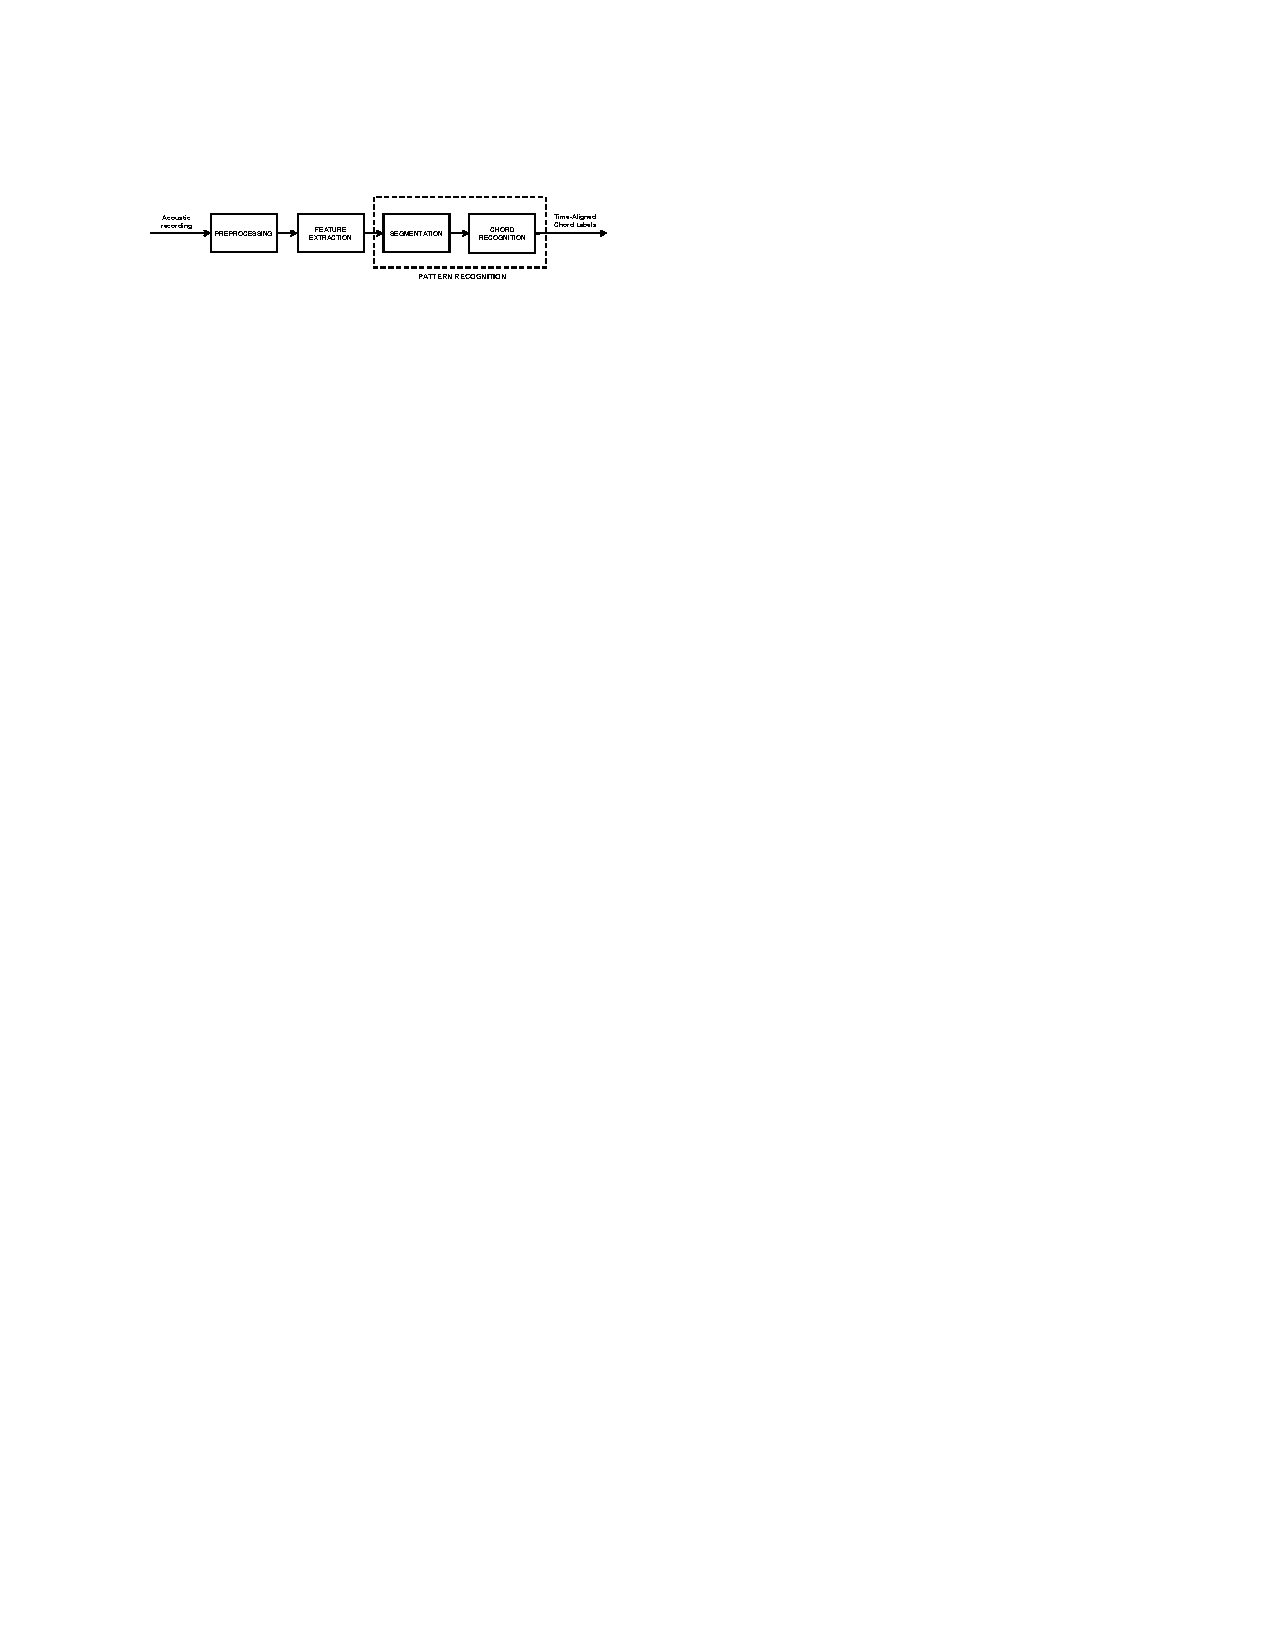
\psfig{file=fig2.pdf,width =5.3in}
\caption{Overview of the chord recognition system used in research case 1~\cite{Morman:2006}.}
\label{fig:fig2}
\end{figure*}  

\section{Background}
In order to explain the process of automatic chord recognition, some general information about feature extraction and pattern matching is needed.

\subsection{Feature Extraction}

The first step of generating a chord progression from audio data is processing the signal to extract harmonic features. Feature extraction is a fairly simple process, but can become more complex due to the addition of optimization steps to increase accuracy \cite{McVicar:2014}. Preprocessing is one of these steps, performed during feature extraction, which results in a \textit{Pitch Class Profile} (PCP), representing what notes are present over time.

\subsubsection{Preprocessing}

In Figure~\ref{fig:fig4}, the light areas show where frequencies have been detected, and the dark areas show empty space. It is clear that frequencies other than just the chord tones have been detected because the light areas are not solid white and the dark areas not solid black. The goal of preprocessing is to reduce as much of this background noise as possible from the audio file, in an effort to provide a smooth and clear PCP. Another issue is that musical instruments produce a series of harmonics at higher and lower frequencies than the tone that is played. These tones, called overtones, can confuse feature extraction techniques, so they need to be removed. These two issues, background noise and overtones, are usually addressed separately during preprocessing. \\

%Depending on the audio resolution, very low pitches can be hard to distinguish and tend to blur across multiple pitches. Percussion sounds also need to be addressed, especially those that create a pitch such as a bass drum. 

%Preprocessing and pre-/post-filtering are optional steps but all of the systems in this paper use it in some way. The reason is that audio files are not perfect; they contain other tones and frequencies that are unrelated to the chords being played. Musical instruments also produce what are known as overtones, tones that sound above or below the note that was played \cite{TaeMin:2014}. Preprocessing is done to the raw audio file, to remove unwanted noise and frequencies. Pre-filtering is done after the feature extraction step, in order to smooth out the PCP. Post-filtering is done after the chords have been determined by the pattern recognition step, finding the most likely sequence and eliminating unlikely chords.


%\todo[inline]{Explain two types of preprocessing, background spectrum and overtone removal. Explain types and how they work and give more info. Explain more about overtones and how they are detected, give more examples of 'other tones'. the sum of sinusoidal tones of integer multiples of the fundamental frequency. Add a figure.}

\subsubsection{Pitch Class Profile} 

The pitch of a note is measured in two dimensions - height and chroma (pitch class). Height tells which octave a note belongs to, and chroma tells where a note stands within the octave (the name of the note). Height is not a factor in determining chord type because two notes that are an octave apart have the same chroma value. A chromagram, or PCP, is a 12-dimensional vector representation of chroma, representing the intensity of each of the twelve semitones in the chromatic scale, over a period of time. An example of a common PCP, along with the actual progression, can be seen in Figure~\ref{fig:fig4}~\cite{McVicar:2014}. 

For over a decade PCP has been the most popular way to represent harmonic features for chord recognition. Most new approaches are variations or refinements of this approach \cite{TaeMin:2014}. These systems can have many more steps in converting audio to PCP including tuning correction, which compensates for music that is not tuned to standard pitch \textit{A4 = 440 Hz}, and beat-synchronization, which calculates the average pitch between beats to get rid of changes caused by noise and other transients. \cite{McVicar:2014}.

%\todo[inline]{Describe them or some of them. Decide between using pitch class and chroma. More detail in paper 1 under feature extraction}

\begin{figure}
\centering
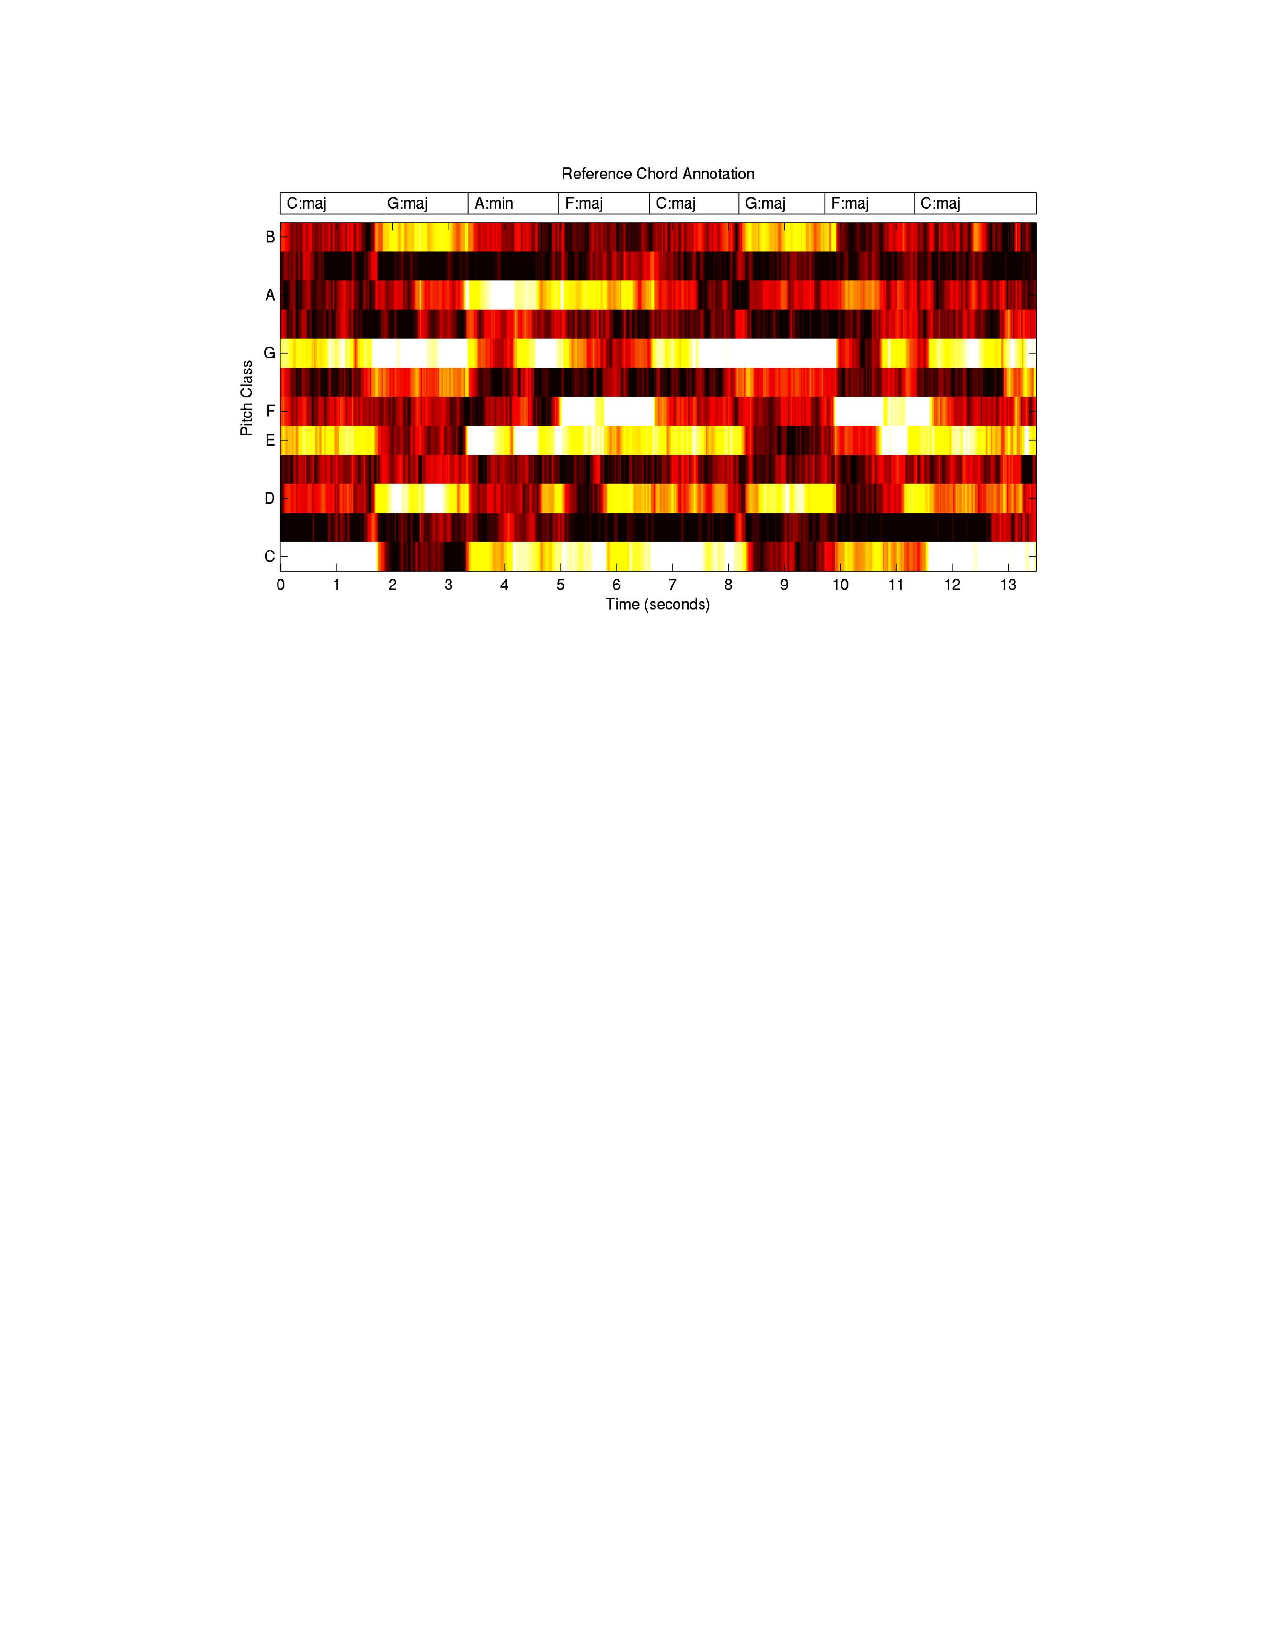
\psfig{file=fig4.pdf,width =3in}
\caption{A typical chromagram, or PCP, generated from the opening to \textit{Let It Be} (Lennon/McCartney). Pitch class (chroma) at time t is shown by the lightness at that point. The true chord progression (simplified) is shown above for comparison.}
\label{fig:fig4}
\end{figure}

\begin{table*}
\centering
\begin{tabular}{|c|c|c|c|c|c|} \hline
 & \textbf{Type} & \textbf{Sample Rate} & \textbf{FFT Length} & \textbf{Liftering} & \textbf{HPS Ratio} \\ \hline
\textbf{FV1} & FB & 44100 & 32768 & yes & 5 \\ \hline
\textbf{FV2} & PCP & 11025 & 4096 & no & 1 \\ \hline
\textbf{FV3} & PCP & 44100 & 32768 & no & 1 \\ \hline
\textbf{FV4} & PCP & 44100 & 32768 & yes & 5 \\ \hline
\end{tabular}
\caption{Feature Vectors, or combinations of methods used for feature extraction, for isolated chord recognition in research case 1~\cite{Morman:2006}.}
\label{tab:tab2}
\end{table*} 

\subsection{Pattern Matching}

Almost all chord recognition systems use PCP or some other chroma-based feature extraction technique. What differentiates these systems is the mechanism used to assign the chord labels. Generating the chord model against which the PCP will be matched can be done either by hand (using musical knowledge), or stochastically (by deriving it from real-world music). The most basic way to model chords is by hand, describing the known note distribution of a chord. An example of a binary chord template (individal chord model) for a C major \textit{triad} (chord containing 3 notes) would look like [1 0 0 0 1 0 0 1 0 0 0 0], where each digit left to right follows the chromatic scale starting at C. A 1 indicates the presence of a note and 0 represents the absence of a note. Using this method, each chord template is created and then tested on each \textit{frame} (time point around 25ms, depending on the system) of a PCP, to find the best fit. The problem with this method is that a lot of times chord tones are not all played at the same time or held for the same duration. More sophisticated chord models are generated stochastically, by defining probability distributions for each chord type that a system can recognize~\cite{TaeMin:2014}.  

%Stochastic chord models are more sophisticated and complex. HMMs used to be the method of choice, but many recent systems prefer Gaussian mixture models \cite{TaeMin:2014}.

%\todo[inline]{Need description of stochastic chord models.}

\subsubsection{Hidden Markov Models}\label{main} 

A \textit{hidden Markov model} (HMM) is a statistical model which describes a finite set of states, in this case chords. Since we do not know the chord progression for a given audio file, these states are considered to be hidden, the observed states are the PCP frames. Transitions between these states are given probabilities that describe the likelihood of transitioning from one state (chord) to another. In the research cases reviewed in this paper, \textit{supervised} HMMs are used, meaning that these probabilities are~\textit{learned} from a set of labeled training data (audio that has been assigned chord labels by hand or some other system)~\cite{wiki:hmm}. The chord transition probabilities are learned for a chord by dividing the number of transitions to each chord by the total number of transitions from that chord. This is done for each chord in the training data. An example of transition probabilities from the C major chord can be seen in Figure~\ref{fig:fig5}. The Viterbi algorithm is then used, which estimates the the best previous chord for each frame recursively, storing the paths in a table. Using the observed states and known transition probabilities, the most likely sequence is estimated and unlikely transitions are restricted~\cite{TaeMin:2014}.

%Need part on how the viterbi algorithm uses the chord models and transition probabilities.

\begin{figure}
\centering
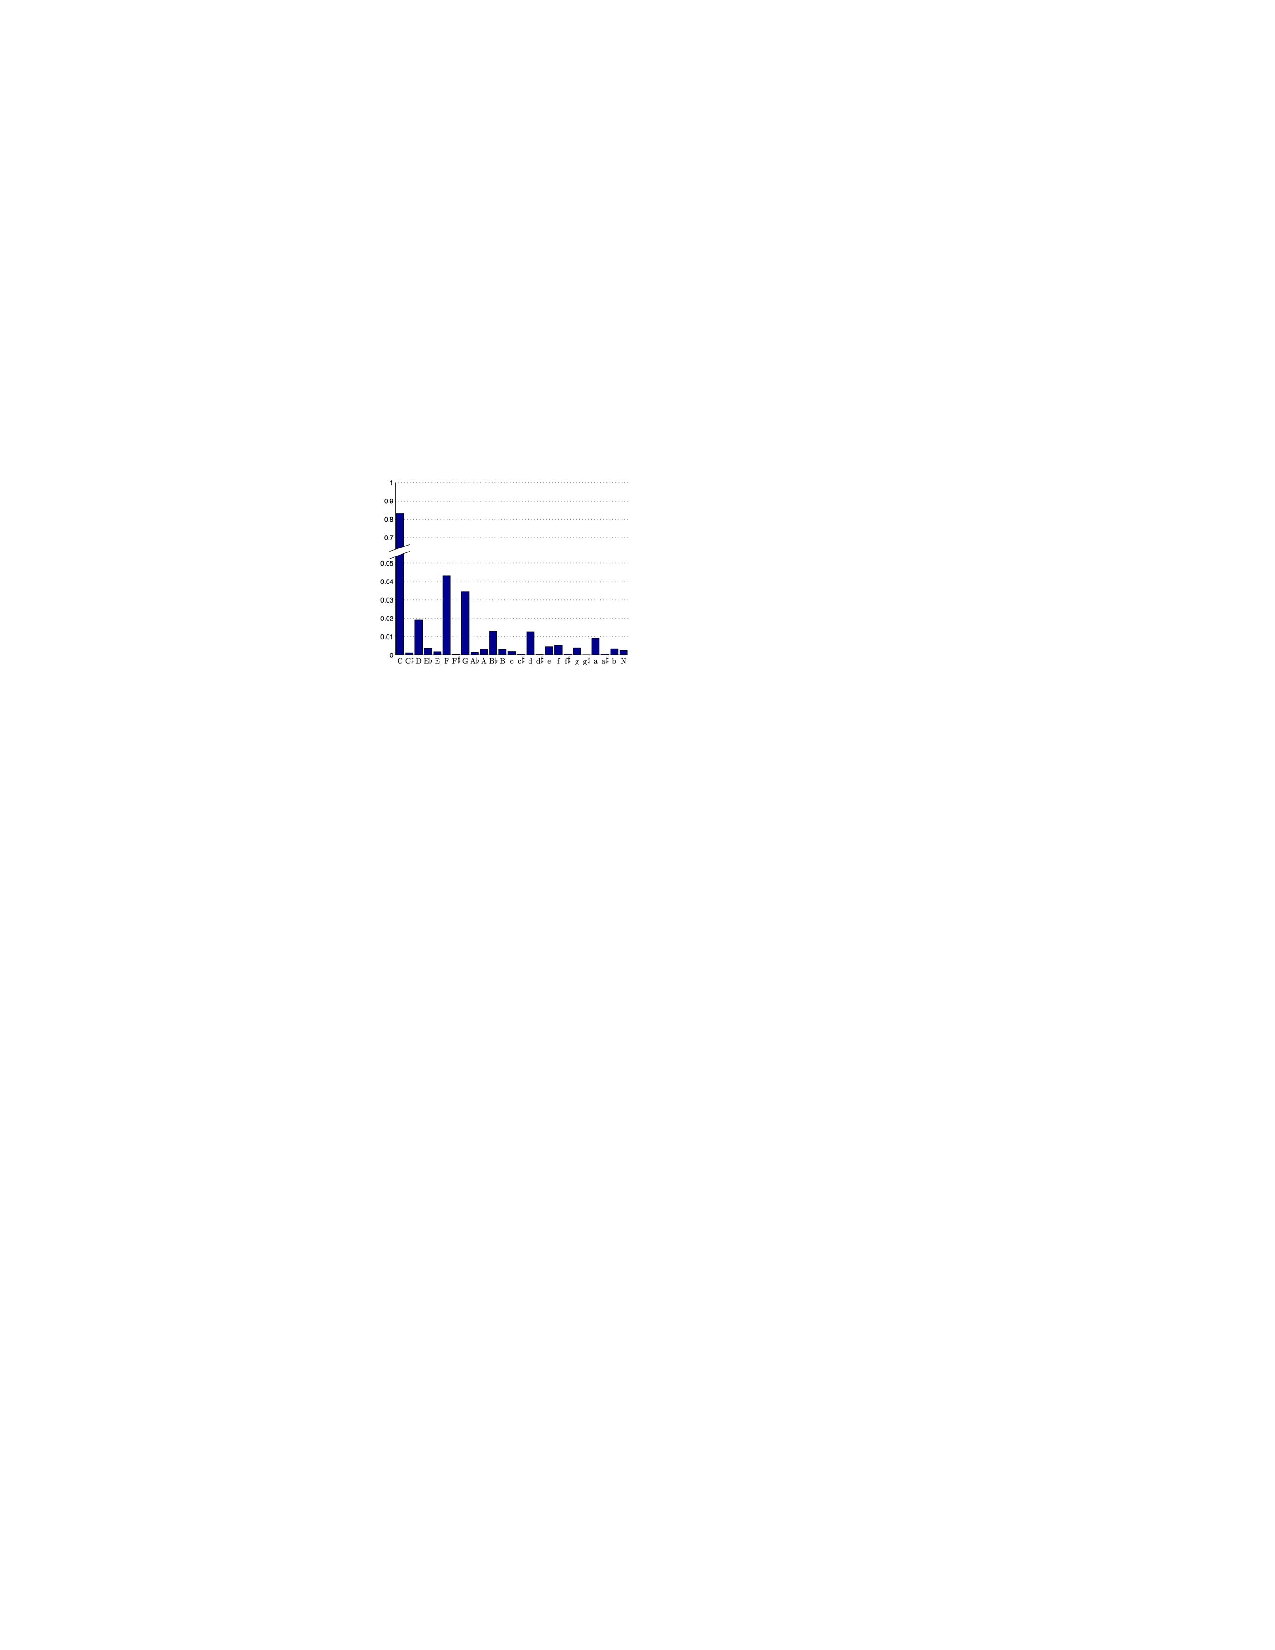
\psfig{file=transitionProbabilities.pdf,width =2.5in}
\caption{An example of transition probabilities from the C major triad, learned from training data.}
\label{fig:fig5}
\end{figure}

%A matrix is created that shows the number of transitions from each chord in the training data to each other possible chord, including itself.

%Transitions between these states are governed by a set of transition probabilities that describe the likelihood of transitioning from one to another. The Viterbi algorithm finds the most likely sequence of these states by evaluating the joint probability of the output and all possible chord sequences, reducing unlikely transitions~\cite{TaeMin:2014}. HMMs are used in a wide variety of pattern recognition environments such as speech, handwriting, gesture recognition, and bioinformatics. 

%\todo[inline]{Need to explain how training works in a more general sense.}

%\todo[inline]{Need to re-write this section from draft. Include figures for models. find first instance of HMM. More info in overview of state of the art.}

\subsubsection{Gaussian Mixture Models}

In a \textit{Gaussian mixture model} (GMM), more detailed models for each chord type are created by averaging multiple PCPs for that type. This is done for each chord type for each of the 12 notes. Multiple Gaussian \textit{components} are also used, which represent different variations of the same chord (i.e., chords with notes excluded or doubled up), providing a more accurate fit. The fit of a frame is measured by the likelihood of a model for that frame. 

%The number of PCPs used to calculate the average is the number of Gaussian components. Models that are created using more than one component are known as GMMs. 

For GMM training, PCPs from the training data are segmented by chord type (i.e., 12 major, 12 minor, depending on what chords are being recognized). To increase the number of training samples, all PCP values for these segments are rotated so that the \textit{root} (name) is C. These segments are then averaged to create models for C-major and C-minor chords, which are then copied and shifted for the remaining 11 keys~\cite{McVicar:2014}.


%\textit{Gaussian mixture models} (GMMs) are used in many modern chord recognition systems. A GMM consists of a distribution of weighted components. Different Gaussian components represent descriptions of each chord in the training data. To train these models, the PCPs from the training data are segmented based on their type; major, minor, or no-chord. These segments are then transposed to all C-based chords (C-major and C-minor). These normalized chords are used to train the C-major and C-minor models, and then re-transposed to the remaining 11 keys~\cite{TaeMin:2014}.

\subsubsection{Support Vector Machines}

\textit{Support Vector Machines} (SVMs) are another type of supervised learning model used for pattern matching. Given a set of labeled training data, SVMs assign labels to segments of the test data. A full explanation of SVMs is outside the scope of this paper, as they are only used in one research case for comparison. Many systems use existing tools for SVM classification.

\section{Research Cases}

This paper looks at three research cases that involve automatic chord recognition. All of these cases include feature extraction and pattern matching. Here we will give an overview of each system, the datasets that were used, and a summary of the results.


\subsection{Case 1: Effects of Proper Signal \\ Processing}

The first research case~\cite{Morman:2006} uses a chord recognition system that begins with a preprocessing block, followed by feature extraction, where the PCP is calculated. After this, the signal is segmented along predicted chord boundaries, and then chord labels are assigned to each segment (pattern matching). An overview of this system can been seen in Figure~\ref{fig:fig2}. 

There are two stages in the preprocessing block, to address background noise and overtones. The first step, Homomorphic Liftering, is a method of separating out the frequencies of musical tones from background and system noise. This is done by finding strong frequency peaks in areas corresponding to the pitch range of the notes. Frequencies above and below a specified range can also be removed to reduce noise. The second step, known as the \textit{Harmonic Product Spectrum} (HPS), is a method which emphasizes frequencies when their overtones are present. HPS is calculated by compressing the spectrum by factors of 1 to R (i.e., 1:2 compression ratio) and multiplying the resulting compressed spectra. The resulting output energy is then summed according to pitch class before a PCP is created.

%\todo[inline]{Explain HPS better.}

The first step of pattern matching for this system is chord segmentation, where the audio signal is segmented at the boundaries where chords change. This can be difficult when the notes of a chord are not played all at once or not held for the same length. To find the points where change has occurred the PCP is analyzed frame-by-frame to find significant change in pitch-class content. 

%FV1 doesn't use PCP

The next and final step in this system is assigning chord labels to the segments. Given an instance of the PCP for a region of the audio, the most probable chord label is picked from a set of training PCPs. In this research case the use of GMMs and SVMs are compared for classification. For SVM classification, a tool called the OSU SVM Classifier MATLAB Toolbox was used (as explained in~\cite{Morman:2006}).

\subsubsection{Datasets}

In this case \textit{Musical Instrument Digital Interface} (MIDI) data was used to create the audio. Two datasets were used: one of isolated chords synthesized on piano and strings, and one of continuous single-instrument music synthesized on piano. 

The isolated chord dataset consisted of 7790 chords and inversions (where the notes are stacked in a different order). Three chord complexity levels were tested, labeled DS1, DS2, and DS3 (seen in Table~\ref{tab:tab1}). DS1 involved the four common triad types (major, minor, augmented, and diminished), across all 12 notes. No other chords were used in DS1. DS2 added variations of the \textit{7th chord} (chords containing four notes): major 7th, minor 7th, dominant 7th, fully diminished 7th, and half diminished 7th. In DS3 all 11 different chord types that the system could recognize were used.

Four \textit{Feature Vectors}~(FV), or combinations of methods used for feature extraction, were compared on each of these complexity levels, seen in Table~\ref{tab:tab2}. FV1 started with preprocessing using homomorphic liftering with a lower cutoff of 30Hz and upper frequency cutoff of 4kHz, then computing HPS with a compression ratio R = 5. Instead of PCP, FV1 uses an 84 dimensional vector (representing 7 octaves with 12 notes per octave). The hypothesis was that this would provide more information because the octaves weren't flattened down to one. FV2 had a lower sampling rate (audio quality), shorter \textit{Fast Fourier Transform}~(FFT) window length (used in converting audio to frequency domain), and no preprocessing was performed on the audio signal. This feature vector was chosen to match a previous system that was being comparing against. FV3 increases the sample rate and FFT, but still leaves out preprocessing. FV4 introduces preprocessing using the same homomorphic liftering and HPS as FV1.

%\todo[inline]{Need more info here. Define/name column headers. Explain table 2 and use the same terminology here.}

The continuous single-instrument audio dataset consisted of 50 hymn verses selected from the Trinity Hymnal, a MIDI collection of 761 hymns, synthesized on piano. 40 were used for training and 10 for testing. Labels similar to DS3 were used, with the exception of 7 Sus. 4, Full Dim., and Half Dim. chords, as they were not common in the dataset. FV4 was used as the feature vector~\cite{Morman:2006}. 

%In the experiments two pattern recognition methods are compared: GMMs and Support Vector Machines (SVM). For SVM classification, the OSU SVM Classifier MATLAB Toolbox was used. 

%\todo[inline]{Explain SVM in a separate section or leave out.}

\begin{table}
\centering
\begin{tabular}{|c|c|c|c|} \hline
&\multicolumn{3}{|c|}{\textbf{Label given in:}} \\ \hline
\textbf{Chord Label} & \textbf{DS1} & \textbf{DS2} & \textbf{DS3} \\ \hline
Major & Major & Major & Major \\ \hline
Minor & Minor & Minor & Minor \\ \hline
Major 7 & - & Major & Major 7 \\ \hline
Minor 7 & - & Minor & Minor 7 \\ \hline
Dom. 7 & - & Major & Dom. 7 \\ \hline
Dim. & Dim. & Dim. & Dim. \\ \hline
Full Dim. & - & Dim. & Full Dim. \\ \hline
Half Dim. & - & Dim. & Half Dim. \\ \hline
Augmented & Aug. & Aug. & Augmented \\ \hline
Sus. 4 & - & - & Sus. 4 \\ \hline
7 Sus. 4 & - & - & 7 Sus. 4 \\ \hline
\end{tabular}
\caption{Chord complexity levels used in research case 1~\cite{Morman:2006}.}
\label{tab:tab1}
\end{table} 

\subsubsection{Results}

For the isolated chords dataset, this system was trained using chords synthesized on a piano, and was tested on chords synthesized on both piano and on strings. The dataset was randomly divided with 80\% of the chords used for training and 20\% for testing. Five of these training and testing sets were created and the recognition rates from these were averaged. The overall chord recognition accuracies for GMMs can be seen in Table~\ref{tab:tab3} for piano, and in Table~\ref{tab:tab4} for strings. FV4 performed the best with the chords played on strings, and showed the least difference between recognizing piano and string chords \cite{Morman:2006}. The results of classification using SVMs can be seen in Table~\ref{tab:tab7}. Using SVMs clearly outperformed GMMs when tested with the instrument that they were trained with, yielding accuracy rates up to 95\%. This was not the case however, when SVMs were tested on strings when trained on piano. In this case SVMs actually did not work because an SVM requires knowledge of the type of data in the testing set, so these results were not included.  

For the continuous single-instrument dataset, the number of \textit{scatter points} (7 scatter points means the partition frame plus 3 frames on each side) were compared, as shown in Table~\ref{tab:tab8}. Recognition accuracy of around 88\% was achieved. Melody tones that were not part of the chord made this more difficult than labeling the isolated chords~\cite{Morman:2006}. 



\begin{table}[h]
\centering
\begin{tabular}{|c|c|c|c|} \hline
\textbf{Feature Vector} & \textbf{DS1A} & \textbf{DS1B} & \textbf{DS1C} \\ \hline
\textbf{FV1} & 83.68 & 61.85 & 57.24 \\ \hline
\textbf{FV2} & 90.33 & 82.44 & 82.26 \\ \hline
\textbf{FV3} & \textbf{91.76} & 84.20 & 84.09 \\ \hline
\textbf{FV4} & 85.64 & 79.40 & 78.93 \\ \hline
\end{tabular}
\caption{Isolated chord recognition accuracy using GMM, training set: piano, testing set: piano~\cite{Morman:2006}.}
\label{tab:tab3}
\end{table} 

\begin{table}[h]
\centering
\begin{tabular}{|c|c|c|c|} \hline
\textbf{Feature Vector} & \textbf{DS1A} & \textbf{DS1B} & \textbf{DS1C} \\ \hline
\textbf{FV1} & 68.06 & 42.00 & 33.62 \\ \hline
\textbf{FV2} & 42.72 & 18.60 & 16.30 \\ \hline
\textbf{FV3} & 43.49 & 22.00 & 18.31 \\ \hline
\textbf{FV4} & \textbf{86.94} & 80.23 & 80.18 \\ \hline
\end{tabular}
\caption{Isolated chord recognition accuracy using GMM, training set: piano, testing set: strings~\cite{Morman:2006}.}
\label{tab:tab4}
\end{table}

\begin{table}[h]
\centering
\begin{tabular}{|c|c|c|c|} \hline
\textbf{Feature Vector} & \textbf{DS1A} & \textbf{DS1B} & \textbf{DS1C} \\ \hline
\textbf{FV1} & 93.43 & 88.21 & 86.52 \\ \hline
\textbf{FV2} & 94.78 & 93.26 & 93.13 \\ \hline
\textbf{FV3} & \textbf{95.23} & 94.31 & 94.24 \\ \hline
\textbf{FV4} & 90.56 & 88.08 & 87.74 \\ \hline
\end{tabular}
\caption{Isolated chord recognition accuracy using SVM, training set: piano, testing set: piano~\cite{Morman:2006}.}
\label{tab:tab7}
\end{table}

\begin{table}[h]
\centering
\begin{tabular}{|c|c|c|c|} \hline
\multicolumn{4}{|c|}{\textbf{Number of Scatter Points}} \\ \hline
\textbf{3} & \textbf{5} & \textbf{7} & \textbf{9} \\ \hline
72.73 & 87.77 & 88.07 & \textbf{88.42} \\ \hline
\end{tabular}
\caption{Continuous single-instrument recognition accuracy with varying number of scatter points~\cite{Morman:2006}.}
\label{tab:tab8}
\end{table}

\begin{figure}[h]
\centering
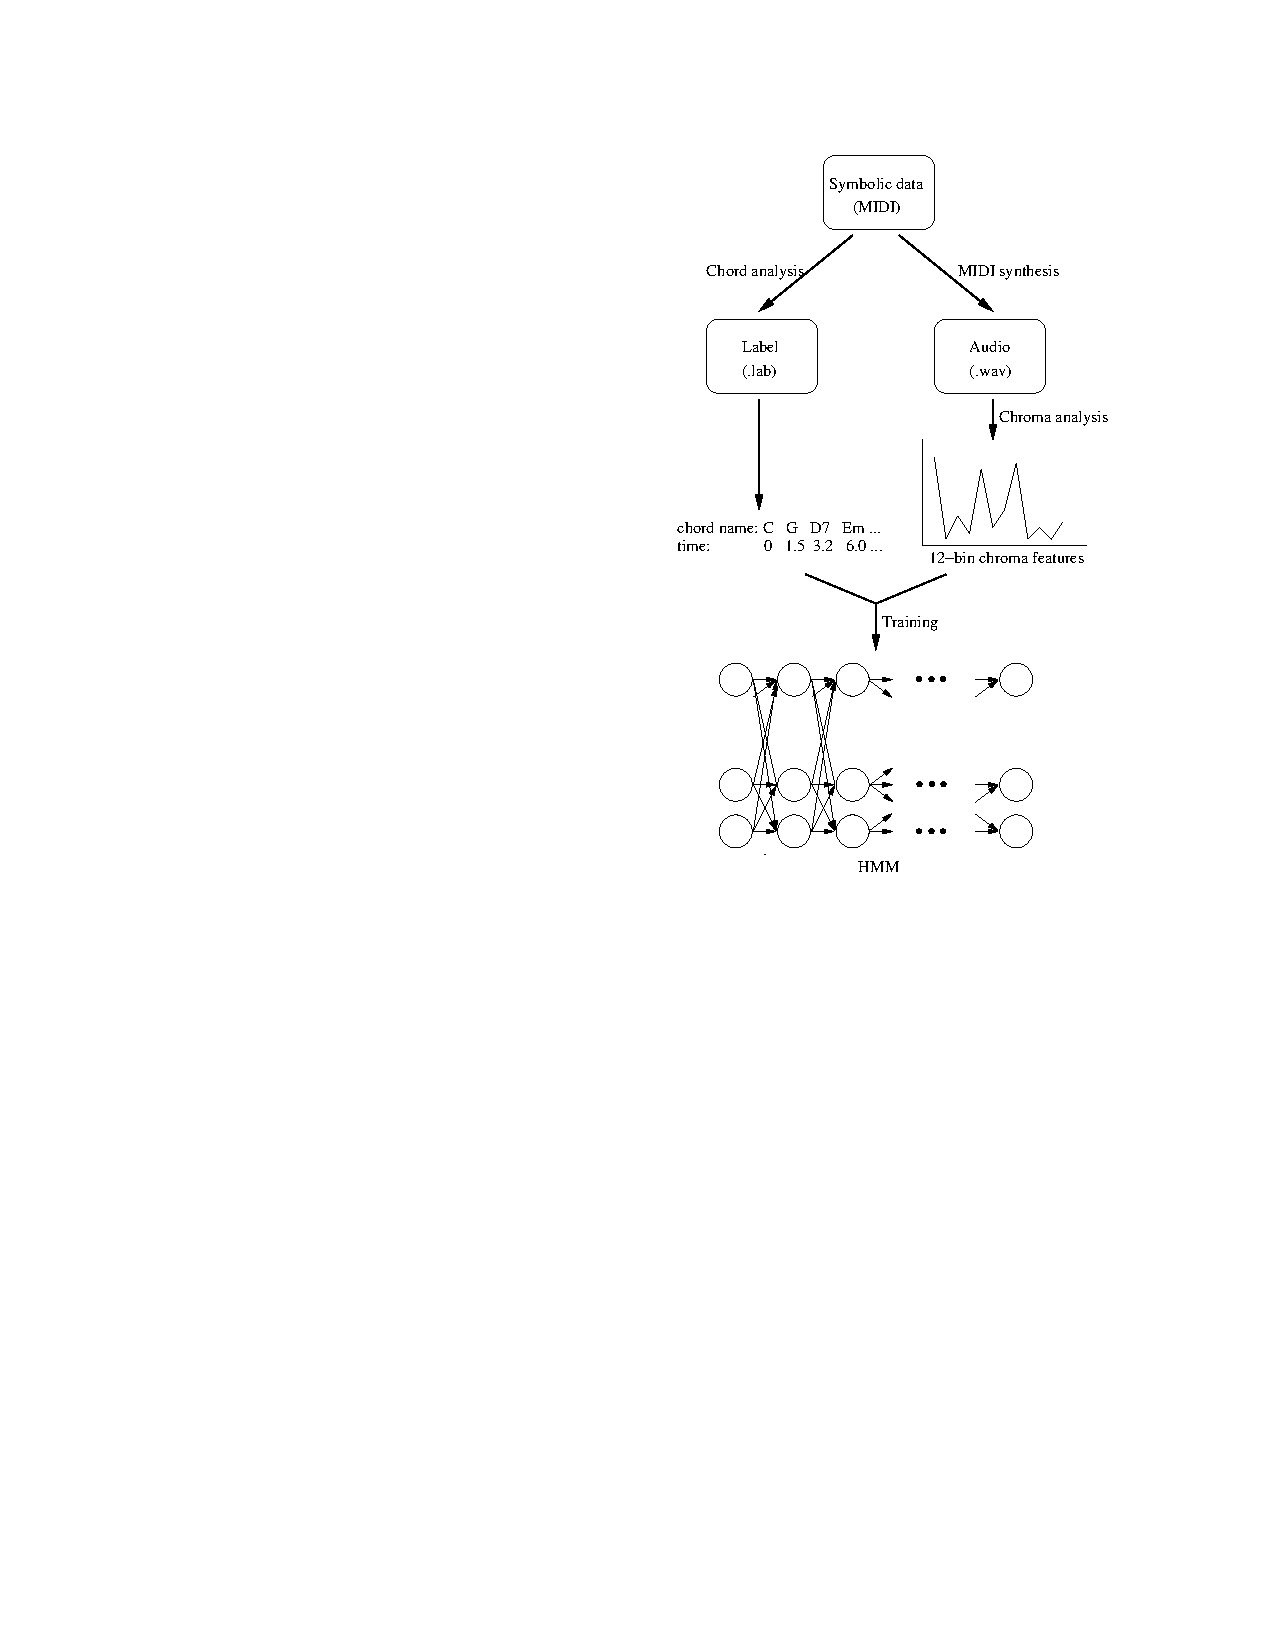
\psfig{file=fig1.pdf,width =3in}
\caption{Overview of the HMM trained with audio from symbolic data in research case 2~\cite{Lee:2006}.}
\label{fig:fig1}
\end{figure}

\subsection{Case 2: HMM Trained with Audio from Symbolic Data}

In the next research case~\cite{Lee:2006}, symbolic data in Humdrum data format is used to generate training data for an HMM. Humdrum is a software toolkit used for music research. The data is used to generate a chord label file (containing chord names and times), and an audio file (synthesized from MIDI), from the same data. Chroma analysis is then performed on the audio file to get a PCP, which is used as input to the trained HMM along with the chord label file. This system is visualized in Figure~\ref{fig:fig1}.

A 36-state HMM is used, with each state representing a chord (major, minor, and diminished for each 12 pitches). Once the model parameters are learned, the Viterbi algorithm is applied to find the optimal sequence in a maximum likelihood sense. 

%At the same time, chord label data is generated from the MIDI data that was used to generate the audio. This data is used to train a 36-state HMM \cite{Lee:2006}. These 36 states represent 36 chords - major, minor, and diminished for each 12 notes. The system is trained on a dataset, and then fed a separate dataset for testing and analysis.

%Using an ergodic model, which allows every possible transition from chord to chord, the model parameters are learned, and then the Viterbi algorithm is applied. The Viterbi algorithm finds the most likely path, or chord sequence, by restricting unlikely chord transitions \cite{TaeMin:2014}. Two elements are needed to train this model: chord label files, and audio data. In this case they are both being generated from the same symbolic data. See figure~\ref{fig:fig1} for a representation of this. The first step is to use a chord analysis tool to generate a file with complete chord information for a piece of music. Using the same symbolic data, the audio files are generated using a sample-based synthesizer. This audio data is in perfect sync with the chord label file, and simulates a real recording because it contains the overtones that would be generated from real instruments \cite{Lee:2006}.

%\todo[inline]{Need to re-write from section draft! More on Viterbi.}



\subsubsection{Datasets}

Two training datasets were used: the first consisted of 81 solo piano pieces by J.S. Bach, Beethoven, and Mozart, and the second consisted of 196 string quartet pieces by Beethoven, Haydn, and Mozart. For the testing datasets, five piano solos and five string quartet pieces were selected from the Kostka and Payne's book, which includes hand-marked analysis and audio recordings done by the composers. Both of these sets were tested using both of the training datasets, as well as third that consisted of the first two combined, resulting in six possible training - testing pairs. The output of the system was compared to the hand-marked data to check for accuracy~\cite{Lee:2006}. 

\subsubsection{Results}

The results of the experiments in this case can be seen in Table~\ref{tab:tab5}. The recognition rate was highest for the combined training dataset, at 80\%, although the difference is not significant. Further analysis on the results showed that the highest error came from non-chord tones in the melody, especially in faster pieces. This is because the analysis window would span over multiple chord changes, which confused the system. Other issues were caused by the system treating 7th chords the same as triads because 7th chords contain two triads.

\begin{table}[h]
\centering
\begin{tabular}{|c|c|c|} \hline
\textbf{Training Data} & \textbf{Test Data} & \textbf{Recognition Rate} \\ \hline
Piano & Piano & 68.69 \\ \hline
String Quartet & Piano & 73.40 \\ \hline
Piano \& Strings & Piano & 74.41 \\ \hline
Piano & String Quartet & 79.35 \\ \hline
String Quartet & String Quartet & 79.76 \\ \hline
Piano \& Strings & String Quartet & \textbf{80.16} \\ \hline
\end{tabular}
\caption{Recognition results for all six possible training - test pairs in research case 2~\cite{Lee:2006}.}
\label{tab:tab5}
\end{table}

\begin{table*}
\centering
\begin{tabular}{|c|c|c|c|c|} \hline
\textbf{Expt.} & \textbf{Highest Accuracy} & \textbf{Pre-filtering} & \textbf{Pattern Matching} & \textbf{Post-filtering} \\ \hline
1 & 58.30 & - & 1 Gaussian component & - \\ \hline
2 & 71.22 & Moving average filters & 1 Gaussian component & - \\ \hline
3 & \textbf{77.90} & - & 25 Gaussian components & HMM \\ \hline
4 & 77.58 & Moving average filters & 25 Gaussian components & HMM \\ \hline

\end{tabular}
\caption{Results from research case 3~\cite{TaeMin:2014}, showing the highest accuracy in each experiment, and the components used to achieve it.}
\label{tab:tab9}
\end{table*}

\subsection{Case 3: Importance of Individual \\ Components}

The final research case~\cite{TaeMin:2014} consists of four experiments, testing different methods used for each step of the process. The overall recognition system in this case is defined as a feature extraction step and pattern matching step, with optional pre-filtering and post-filtering steps. In this case preprocessing is part of the feature extraction step. An overview of the system can been seen in Figure~\ref{fig:fig3}. Pre-filtering is applied to PCPs directly before pattern matching, and consists of averaging frames between beats, yielding a beat-synchronized PCP. Post-filtering is performed after pattern matching, in the form of an HMM using a Viterbi decoder.

In the first experiment, different combinations of chroma features and chord models were tested to show whether or not model complexity affects performance of the system. The second experiment looked at the effect of different pre-filtering techniques, while the third looked at the effect of post-filtering. The fourth experiment used both pre-filtering and post-filtering, in all possible parameter combinations.
%The final study \cite{TaeMin:2014} compares the most common methods of each step: feature extraction, pattern recognition, and pre/post filtering. This study describes the overall system a little differently than the other two, with preprocessing included in the feature extraction stage, and HMMs included in the post-filtering stage. The pre-filtering stage is where attempts are made to smooth out the PCP. 

%Four experiments were conducted in this study: Feature extraction and pattern matching, effect of pre-filtering, effect of post-filtering, and combined pre- and post-filtering. Each experiment was run on 495 chord annotated pop songs. 

%In the first experiment, different combinations of feature extraction and pattern matching are compared to show whether or not model complexity affects performance of the system. They also test the effect of different types of chroma features. The second experiment looks at the pre-filtering techniques of moving filters and beat-synchronization. \todo[inline]{Need to define these and provide more here.} The effect of post-filtering experiment compares the use of different stochastic models. The final experiment uses pre- and post-filtering and again looks at moving filters and beat-synchronization.

\begin{figure}[h]
\centering
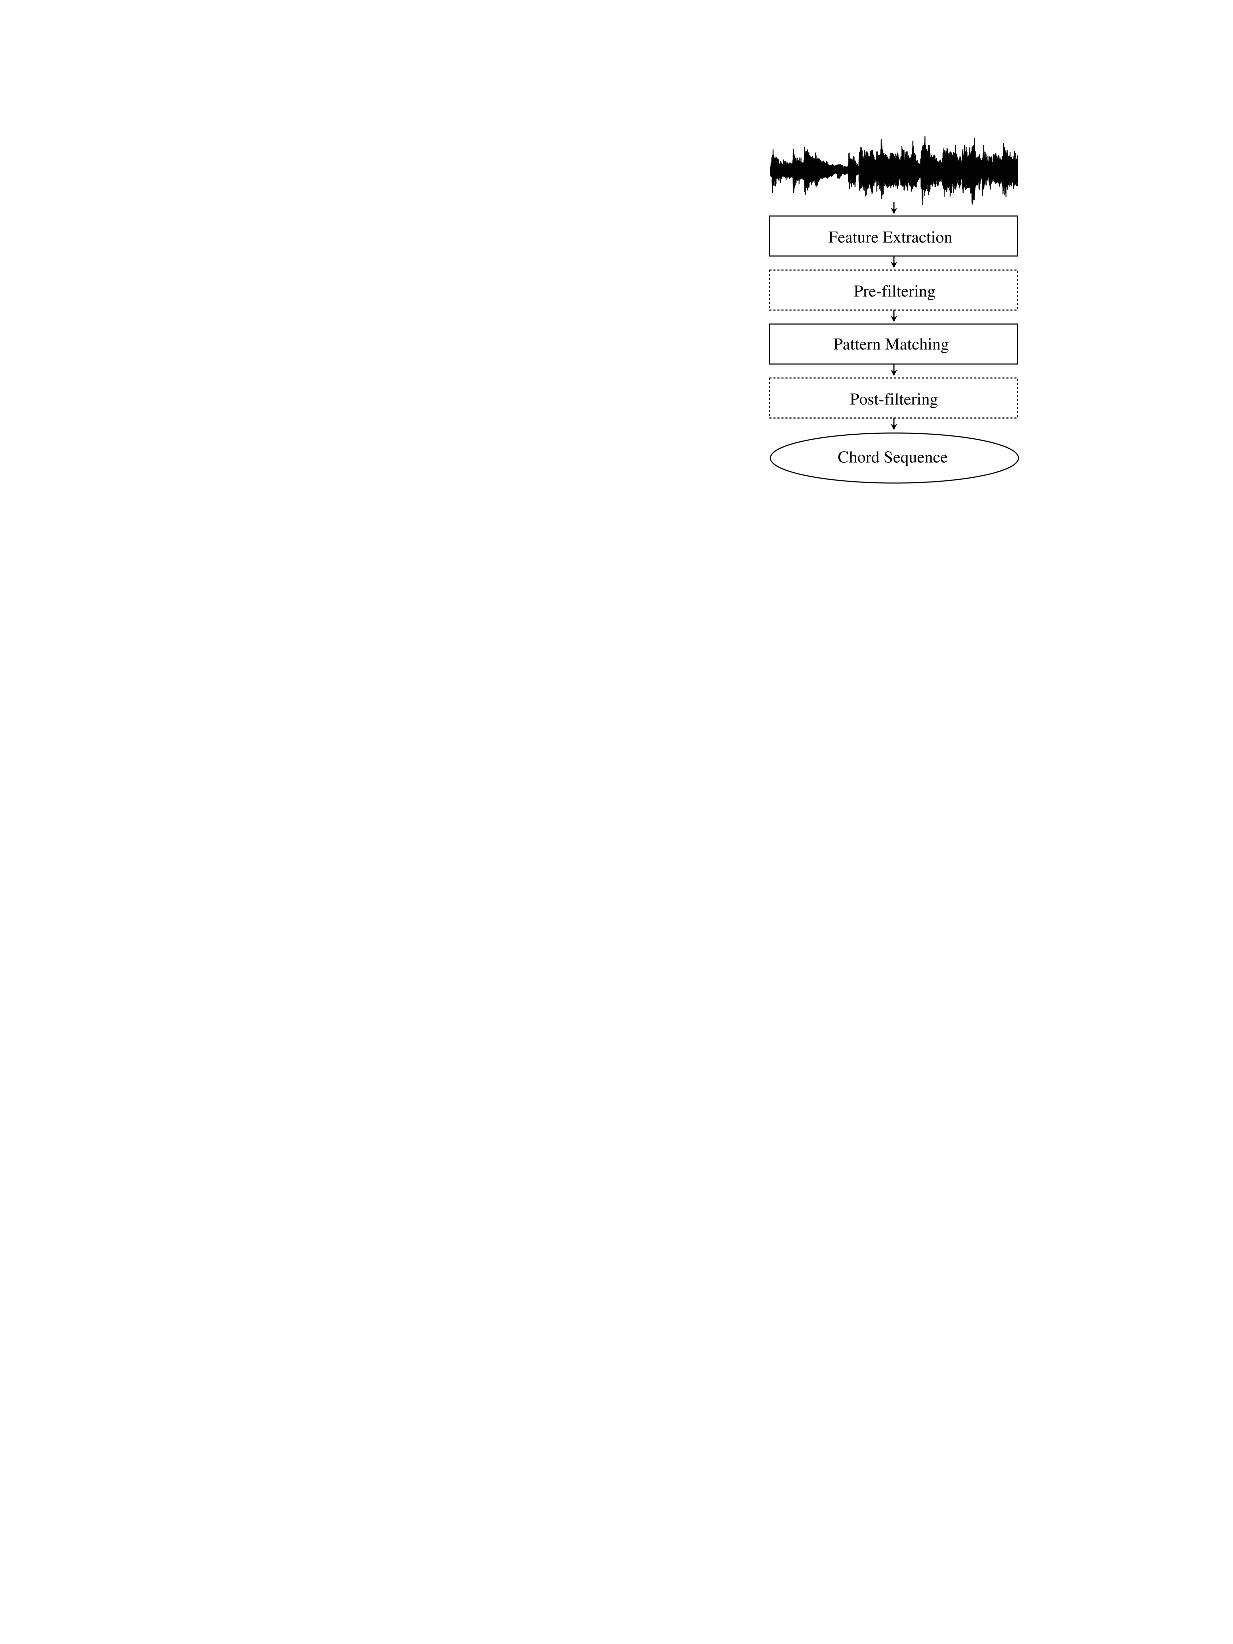
\psfig{file=fig3.pdf,height=2.5in}
\caption{General layout of the chord recognition system used in research case 3~\cite{TaeMin:2014}. In this case preprocessing is included in the feature extraction step.}
\label{fig:fig3}
\end{figure}

\subsubsection{Datasets}

Each of the four experiments in this research case were performed on 180 Beatles songs, 20 Queen songs, 100 songs from the RWC (Real World Computing) pop dataset, and 195 songs from the US-Pop dataset, for a total of 495 songs. The RWC and US-Pop dataset were assigned chord labels by hand, while the Beatles and Queen chord models were generated stochastically. For training, 5-fold cross validation was used with each group having 99 songs selected randomly. For each fold one group is selected and the other four are used for training. Accuracy is represented by the total duration of correct chords out of the total duration of the dataset~\cite{TaeMin:2014}.

\subsubsection{Results}

The results of the four experiments conducted in this case can be seen in Table~\ref{tab:tab9}. In all four experiments the best results were found using a combination of these two preprocessing methods: de-emphasizing high and low frequencies and using log compression, which limits the dynamic range caused by multiple instruments at different volumes. Each experiment was also tried using 1, 5, 10, and 25 Gaussian components, to test if a more complex chord model would increase accuracy. For each experiment the best result and components used to achieve it are shown in Table~\ref{tab:tab9}. 

In the first experiment, no filtering was applied during the process. This experiment was testing the difference between preprocessing techniques in the feature extraction stage (the best combination is mentioned above). We would expect to see higher accuracy with more Gaussian components used, but that was not the case in this experiment, where the best score was found by using only one component. The highest error was in distinguishing major and minor chords with the same root, because two of the notes are shared and the third is only a half-step different. For the second experiment, pre-filtering was applied using \textit{moving average filters}, which look for noisy frames and smooth them across the neighboring frames. The highest accuracy in this experiment was again achieved by using only one Gaussian component. The third experiment used post-filtering with no pre-filtering, and here we see that the best performance was achieved by using more Gaussian components. This is because post-filtering is dependent on the probability values for different chord models. The final experiment, using both pre-filtering and post-filtering, showed about the same result as post-filtering alone. This is because moving average filters sometimes did too much smoothing and ended up blurring out chord boundaries and other signal detail.

%The binary template is the hand-made chord model, and the rest are GMMs with a number indicating the number of Gaussian components used. We would expect to see higher accuracy with more processing and more Gaussian components used, but this is not the case. The highest error was in distinguishing major and minor chords with the same root, because two of the notes are shared and the third is only a half-step different.

%Re-make this table as comparing the 4 experiments, the highest result, and what was used to obtain it.




%\begin{table*}
%\centering
%\begin{tabular}{|c|c|c|c|c|c|c|c|} \hline
% & Binary Template & GMM-1 & GMM-5 & GMM-10 & GMM-15 & GMM-20 & GMM-25 \\ \hline
%Base & 46.95 & 46.46 & 46.26 & 48.10 & 48.39 & 48.74 & 48.77 \\ \hline
%Overtone removal 1 & 52.12 & 49.40 & 47.38 & 50.24 & 51.04 & 51.42 & 51.71 \\ \hline
%Overtone removal 2 & 54.38 & 54.51 & 50.49 & 50.90 & 51.42 & 52.14 & 51.97 \\ \hline
%Timbre Homogenization 1 & 45.18 & 48.24 & 50.44 & 49.34 & 49.36 & 49.06 & 49.35 \\ \hline
%Timbre Homogenization 2 & 44.37 & 40.12 & 39.80 & 39.61 & 40.49 & 40.87 & 40.86 \\ \hline
%OR1 \& TH1 & 55.51 & \textbf{58.30} & 57.58 & 57.73 & 57.72 & 57.70 & 57.69 \\ \hline
%OR1 \& TH2 & 53.24 & 53.83 & 54.66 & 54.67 & 54.00 & 54.03 & 53.55 \\ \hline
%OR2 \& TH1 & 55.00 & 56.29 & 53.09 & 53.24 & 53.28 & 53.33 & 53.43 \\ \hline
%\end{tabular}
%\caption{Average accuracy without filtering (research case 3~\cite{TaeMin:2014}, experiment 1).}
%\label{tab:tab6}
%\end{table*}

%\todo[inline]{Need to add the results for pre and post filtering experiments. Explain table 8 better. Possibly combine all 4 experiments into one table, with the highest accuracy achieved in each and how.}


\section{Conclusions}

The highest accuracy that we see in this paper was around 95\% for the isolated chord dataset using SVMs in~\cite{Morman:2006}. This is more of a proof of concept since these systems are aimed at providing chord data for an entire song. If we look at the results of all experiments tested on continuous music, we see that the highest accuracy achieved was around 88\% for the continuous music dataset in~\cite{Morman:2006}. The components used in this experiment were: preprocessing using homomorphic lifering and HPS with a ratio of R = 5, chord segmentation using SVMs, and chord recognition using SVMs. This was using a relatively small dataset, they mention in~\cite{Morman:2006} that the training procedure for SVMs is very complex with large amounts of data. This implies that the system used for chord recognition is somewhat dependent on the dataset that is being tested. Systems can be tailored specifically to the type of instrument and chords that are present in the dataset.

There are still many issues and pitfalls with these and all chord recognition systems. Music that has a lot of different instruments, fast chord changes, and types of chords that are not recognized can cause significant problems if they are not expected. The pattern matching techniques in this paper assume that individual chords are independent of each other, but in real-world music some chords can only be labeled correctly by the context of the surrounding chords~\cite{TaeMin:2014}. An example is a secondary chord, which is borrowed from another key. These chords would be given a chord label that is not in the key of the song, rather than the secondary label that would be applied by hand. Detecting these and other non-regular chords would be very difficult for these systems, as they only recognize the chords that they are designed for.    

%\todo[inline]{Look at the components of the highest performing systems and determine the best techniques used for feature extraction and pattern matching. Discuss the effects of preprocessing during feature extraction and using HMMs to eliminate unlikely sequences. All of the research cases use PCP and preprocessing of some kind. Case 1 and 3 use GMMs. Case 2 and 3 use HMMs.}

%\todo[inline]{Talk about some of the issues and pitfalls with these and all chord recognition systems. Including dense recordings, extremely fast chord changes, and other types of chords that are not recognized. There are also chords that can only be determined by their context and chords that can be interpreted in more than one way.}

\subsection{Future Work}

With the increasing amount of data that is available online, some systems have been developed that scrape online databases of songs that have already been labeled to use for training data. The advantage here is having a large amount of labeled chord data without having to generate it. The system in~\cite{McVicar:2010} was able to scrape chord information from \texttt{e-chords.com} for over 75,000 songs. There are also genre-specific models, which account for different chord transition probabilities in different genres of music. These models can also be used to identify genre by testing with all of the genre models and selecting the one with the best result~\cite{McVicar:2014}. Progress is being made in this area, including mobile apps that can provide chord data for audio captured with the microphone.

%\todo[inline]{Will be adding a little more here, possibly moving this section before Conclusion.}

\section{Acknowledgements}

Many thanks to Elena Machkasova, KK Lamberty, and Scott Steffes for their invaluable feedback. 

%\subsection{Math Equations}
%You may want to display math equations in three distinct styles:
%inline, numbered or non-numbered display.  Each of
%the three are discussed in the next sections.

%\subsubsection{Inline (In-text) Equations}
%A formula that appears in the running text is called an
%inline or in-text formula.  It is produced by the
%\textbf{math} environment, which can be
%invoked with the usual \texttt{{\char'134}begin. . .{\char'134}end}
%construction or with the short form \texttt{\$. . .\$}. You
%can use any of the symbols and structures,
%from $\alpha$ to $\omega$, available in
%\LaTeX\cite{Lamport:LaTeX}; this section will simply show a
%few examples of in-text equations in context. Notice how
%this equation: \begin{math}\lim_{n\rightarrow \infty}x=0\end{math},
%set here in in-line math style, looks slightly different when
%set in display style.  (See next section).
%
%\subsubsection{Display Equations}
%A numbered display equation -- one set off by vertical space
%from the text and centered horizontally -- is produced
%by the \textbf{equation} environment. An unnumbered display
%equation is produced by the \textbf{displaymath} environment.
%
%Again, in either environment, you can use any of the symbols
%and structures available in \LaTeX; this section will just
%give a couple of examples of display equations in context.
%First, consider the equation, shown as an inline equation above:
%%%%%
%\begin{equation*}
%\lim_{n\rightarrow \infty}x=0
%\end{equation*}
%%%%%
%Notice how it is formatted somewhat differently in
%the \textbf{displaymath}
%environment.  Now, we'll enter an unnumbered equation:
%\begin{displaymath}\sum_{i=0}^{\infty} x + 1\end{displaymath}
%and follow it with another numbered equation:
%\begin{equation}\sum_{i=0}^{\infty}x_i=\int_{0}^{\pi+2} f\end{equation}
%just to demonstrate \LaTeX's able handling of numbering.
%
%\subsection{Multi-line formulas}
%%%%%%% \[ \] denotes math; array environment is needed for multi-line
%%%%%%% format, {c} means that the array has one column, centered 
%%%%%%  (alternatives are {l} for left-aligned, {r} for right-aligned)
%%%%%%  \\ denotes a new line
%\[
%\begin{array}{c}
%n_1 = \sum_{i = 1}^k a_i \\
%n_2 = \prod_{i = 1}^k b_i
%\end{array}
%\]
%
%\subsection{Citations}
%Citations to articles \cite{Morman:2006,Lee:2006,TaeMin:2014} listed
%in the Bibliography section of your
%article will occur throughout the text of your article.
%You should use BibTeX to automatically produce this bibliography;
%you simply need to insert one of several citation commands with
%a key of the item cited in the proper location in
%the \texttt{.tex} file \cite{OM:2008}.
%The key is a short reference you invent to uniquely
%identify each work; in this sample document, the key is
%the first author's surname and a
%word from the title.  This identifying key is included
%with each item in the \texttt{.bib} file for your article.
%
%The details of the construction of the \texttt{.bib} file
%are beyond the scope of this sample document, but more
%information can be found in the \textit{Author's Guide},
%and exhaustive details in the \textit{\LaTeX\ User's
%Guide}.
%
%This article shows only the plainest form
%of the citation command, using \texttt{{\char'134}cite}.
%This is what is stipulated in the SIGS style specifications.
%No other citation format is endorsed or supported.
%
%\subsection{Tables}
%Because tables cannot be split across pages, the best
%placement for them is typically the top of the page
%nearest their initial cite.  To
%ensure this proper ``floating'' placement of tables, use the
%environment \textbf{table} to enclose the table's contents and
%the table caption.  The contents of the table itself must go
%in the \textbf{tabular} environment, to
%be aligned properly in rows and columns, with the desired
%horizontal and vertical rules.  Again, detailed instructions
%on \textbf{tabular} material
%is found in the \textit{\LaTeX\ User's Guide}.
%
%Immediately following this sentence is the point at which
%Table 1 is included in the input file; compare the
%placement of the table here with the table in the printed
%dvi output of this document.
%
%\begin{table}
%\centering
%\caption{Frequency of Special Characters}
%\begin{tabular}{|c|c|l|} \hline
%Non-English or Math&Frequency&Comments\\ \hline
%\O & 1 in 1,000& For Swedish names\\ \hline
%$\pi$ & 1 in 5& Common in math\\ \hline
%\$ & 4 in 5 & Used in business\\ \hline
%$\Psi^2_1$ & 1 in 40,000& Unexplained usage\\
%\hline\end{tabular}
%\end{table}
%
%To set a wider table, which takes up the whole width of
%the page's live area, use the environment
%\textbf{table*} to enclose the table's contents and
%the table caption.  As with a single-column table, this wide
%table will ``float" to a location deemed more desirable.
%Immediately following this sentence is the point at which
%Table 2 is included in the input file; again, it is
%instructive to compare the placement of the
%table here with the table in the printed dvi
%output of this document.
%
%
%\begin{table*}
%\centering
%\caption{Some Typical Commands}
%\begin{tabular}{|c|c|l|} \hline
%Command&A Number&Comments\\ \hline
%\texttt{{\char'134}alignauthor} & 100& Author alignment\\ \hline
%\texttt{{\char'134}numberofauthors}& 200& Author enumeration\\ \hline
%\texttt{{\char'134}table}& 300 & For tables\\ \hline
%\texttt{{\char'134}table*}& 400& For wider tables\\ \hline\end{tabular}
%\end{table*}
%% end the environment with {table*}, NOTE not {table}!
%
%\subsection{Figures}
%Like tables, figures cannot be split across pages; the
%best placement for them
%is typically the top or the bottom of the page nearest
%their initial cite.  To ensure this proper ``floating'' placement
%of figures, use the environment
%\textbf{figure} to enclose the figure and its caption.
%
%This sample document contains examples of %\textbf{.eps}
%%and 
%a \textbf{.pdf} file to be displayable with \LaTeX.  More
%details on each of these is found in the \textit{Author's Guide}.
%
%\begin{figure}
%\centering
%\psfig{file=sample_graph.pdf,width =3in}
%\caption{A sample graph just spanning one column.}
%\end{figure}
%
%
%As was the case with tables, you may want a figure
%that spans two columns.  To do this, and still to
%ensure proper ``floating'' placement of tables, use the environment
%\textbf{figure*} to enclose the figure and its caption.
%\begin{figure*}
%\centering
%\psfig{file=sample_graph.pdf,width =5.3in}
%\caption{A sample graph that needs to span two columns of text.}
%\end{figure*}
%and don't forget to end the environment with
%{figure*}, not {figure}!
%
%It's easiest and you tend to get the best quality if your figures vector graphics
%in PDF format. You can include other formats such as PNG, but they will usually
%not look nearly as professional, especially when printed on high resolution printers.
%\emph{Be vary wary of screen captures from other papers. They tend to look pixelated
%and amateurish even at high resolutions.}
%
%\subsection{Theorem-like Constructs}
%Other common constructs that may occur in your article are
%the forms for logical constructs like theorems, axioms,
%corollaries and proofs.  There are
%two forms, one produced by the
%command \texttt{{\char'134}newtheorem} and the
%other by the command \texttt{{\char'134}newdef}; perhaps
%the clearest and easiest way to distinguish them is
%to compare the two in the output of this sample document:
%
%This uses the \textbf{theorem} environment, created by
%the\linebreak\texttt{{\char'134}newtheorem} command:
%\newtheorem{theorem}{Theorem}
%\begin{theorem}
%Let $f$ be continuous on $[a,b]$.  If $G$ is
%an antiderivative for $f$ on $[a,b]$, then
%\begin{displaymath}\int^b_af(t)dt = G(b) - G(a).\end{displaymath}
%\end{theorem}
%
%The other uses the \textbf{definition} environment, created
%by the \texttt{{\char'134}newdef} command:
%\newdef{definition}{Definition}
%\begin{definition}
%If $z$ is irrational, then by $e^z$ we mean the
%unique number which has
%logarithm $z$: \begin{displaymath}{\log e^z = z}\end{displaymath}
%\end{definition}
%
%Two lists of constructs that use one of these
%forms is given in the
%\textit{Author's  Guidelines}.
% 
%There is one other similar construct environment, which is
%already set up
%for you; i.e. you must \textit{not} use
%a \texttt{{\char'134}newdef} command to
%create it: the \textbf{proof} environment.  Here
%is a example of its use:
%\begin{proof}
%Suppose on the contrary there exists a real number $L$ such that
%\begin{displaymath}
%\lim_{x\rightarrow\infty} \frac{f(x)}{g(x)} = L.
%\end{displaymath}
%Then
%\begin{displaymath}
%l=\lim_{x\rightarrow c} f(x)
%= \lim_{x\rightarrow c}
%\left[ g{x} \cdot \frac{f(x)}{g(x)} \right ]
%= \lim_{x\rightarrow c} g(x) \cdot \lim_{x\rightarrow c}
%\frac{f(x)}{g(x)} = 0\cdot L = 0,
%\end{displaymath}
%which contradicts our assumption that $l\neq 0$.
%\end{proof}
%
%Complete rules about using these environments and using the
%two different creation commands are in the
%\textit{Author's Guide}; please consult it for more
%detailed instructions.  If you need to use another construct,
%not listed therein, which you want to have the same
%formatting as the Theorem
%or the Definition\cite{salas:calculus} shown above,
%use the \texttt{{\char'134}newtheorem} or the
%\texttt{{\char'134}newdef} command,
%respectively, to create it.
%
%\subsection*{A {\secit Caveat} for the \TeX\ Expert}
%Because you have just been given permission to
%use the \texttt{{\char'134}newdef} command to create a
%new form, you might think you can
%use \TeX's \texttt{{\char'134}def} to create a
%new command: \textit{Please refrain from doing this!}
%Remember that your \LaTeX\ source code is primarily intended
%to create camera-ready copy, but may be converted
%to other forms -- e.g. HTML. If you inadvertently omit
%some or all of the \texttt{{\char'134}def}s recompilation will
%be, to say the least, problematic.
%
%\section{Conclusions}
%This paragraph will end the body of this sample document.
%Remember that you might still have Acknowledgments or
%Appendices; brief samples of these
%follow.  There is still the Bibliography to deal with; and
%we will make a disclaimer about that here: with the exception
%of the reference to the \LaTeX\ book, the citations in
%this paper are to articles which have nothing to
%do with the present subject and are used as
%examples only.
%
%\section{Acknowledgments}
%
%This section is optional; it is a location for you
%to acknowledge grants, funding, editing assistance and
%what have you.
%
%It is common (but by no means necessary) for students to thank
%their advisor, and possibly other faculty, friends, and family who provided
%useful feedback on the paper as it was being written.
%
%In the present case, for example, the
%authors would like to thank Gerald Murray of ACM for
%his help in codifying this \textit{Author's Guide}
%and the \textbf{.cls} and \textbf{.tex} files that it describes.

% The following two commands are all you need in the
% initial runs of your .tex file to
% produce the bibliography for the citations in your paper.
\bibliographystyle{abbrv}
% sample_paper.bib is the name of the BibTex file containing the
% bibliography entries. Note that you *don't* include the .bib ending here.
\bibliography{sample_paper}  
% You must have a proper ".bib" file
%  and remember to run:
% latex bibtex latex latex
% to resolve all references

\end{document}
